\documentclass[tikz,border=5pt]{standalone}
\usepackage[T1]{fontenc}
\usepackage{lmodern,amsmath,amssymb}
\usetikzlibrary{arrows.meta,calc,positioning,fit,backgrounds,shapes.geometric,matrix,decorations.pathreplacing,patterns}
\definecolor{ink}{gray}{0.08}
\definecolor{wash}{gray}{0.965}
\definecolor{soft}{gray}{0.45}
\tikzset{box/.style={draw=ink,line width=.65pt,fill=white,align=center,inner sep=4pt,outer sep=0pt,font=\small},flow/.style={draw=ink,line width=.65pt,-{Latex[length=1.8mm,width=1.3mm]},rounded corners=2pt},annotation/.style={font=\scriptsize,text=soft,align=center},groupbox/.style={draw=soft,dashed,line width=.45pt,fill=wash}}
\begin{document}
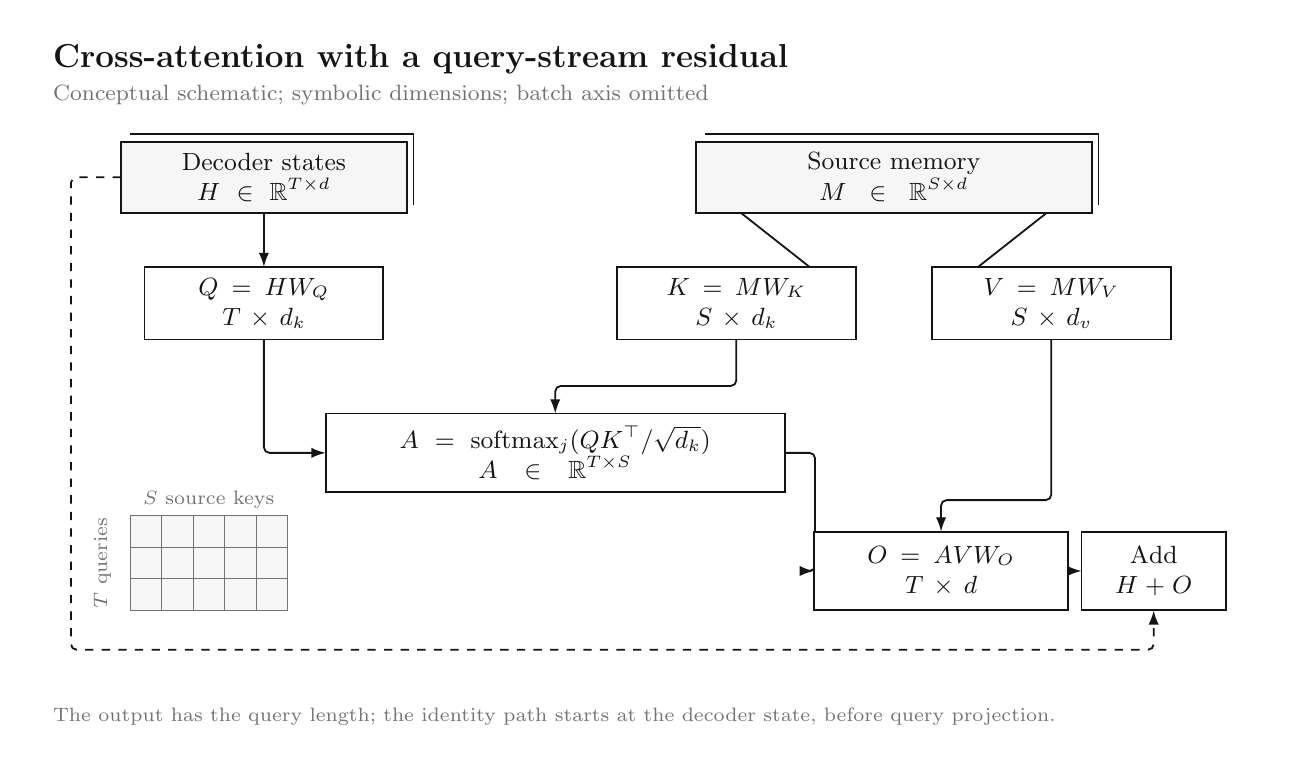
\begin{tikzpicture}[x=1cm,y=-1cm,font=\rmfamily,text=ink]

\path[use as bounding box] (0,0) rectangle (16,9);
\node[anchor=west,font=\large\bfseries] at (.2,.4) {Cross-attention with a query-stream residual};
\node[anchor=west,font=\footnotesize,text=soft] at (.2,.85) {Conceptual schematic; symbolic dimensions; batch axis omitted};
\begin{pgfonlayer}{background}
\end{pgfonlayer}
\node[box,fill=wash,minimum width=3.6cm,minimum height=0.9cm,text width=3.35cm] (h) at (3.0,1.9) {Decoder states\\$H\in\mathbb{R}^{T\times d}$};
\draw[ink,line width=.4pt] (1.3,1.3499999999999999) -- (4.8999999999999995,1.3499999999999999) -- (4.8999999999999995,2.25);
\node[box,fill=wash,minimum width=5.0cm,minimum height=0.9cm,text width=4.75cm] (m) at (11.0,1.9) {Source memory\\$M\in\mathbb{R}^{S\times d}$};
\draw[ink,line width=.4pt] (8.6,1.3499999999999999) -- (13.6,1.3499999999999999) -- (13.6,2.25);
\node[box,minimum width=3.0cm,minimum height=0.9cm,text width=2.75cm] (q) at (3.0,3.5) {$Q=HW_Q$\\$T\times d_k$};
\node[box,minimum width=3.0cm,minimum height=0.9cm,text width=2.75cm] (k) at (9.0,3.5) {$K=MW_K$\\$S\times d_k$};
\node[box,minimum width=3.0cm,minimum height=0.9cm,text width=2.75cm] (v) at (13.0,3.5) {$V=MW_V$\\$S\times d_v$};
\node[box,minimum width=5.8cm,minimum height=1.0cm,text width=5.55cm] (score) at (6.7,5.4) {$A=\operatorname{softmax}_{j}(QK^\top/\sqrt{d_k})$\\$A\in\mathbb{R}^{T\times S}$};
\node[box,minimum width=3.2cm,minimum height=1.0cm,text width=2.95cm] (out) at (11.6,6.9) {$O=AVW_O$\\$T\times d$};
\node[box,minimum width=1.8cm,minimum height=1.0cm,text width=1.55cm] (add) at (14.3,6.9) {Add\\$H+O$};
\begin{pgfonlayer}{background}
\draw[flow] (h.south) -- (q.north);
\draw[flow] (m.west) -- (k.east);
\draw[flow] (m.east) -- (v.west);
\draw[flow] (q.south) -- (3,5.4) -- (score.west);
\draw[flow] (k.south) -- (9,4.55) -- (6.7,4.55) -- (score.north);
\draw[flow] (score.east) -- (10,5.4) -- (10,6.9) -- (out.west);
\draw[flow] (v.south) -- (13,6.0) -- (11.6,6.0) -- (out.north);
\draw[flow] (out.east) -- (add.west);
\draw[flow,dashed] (h.west) -- (0.55,1.9) -- (0.55,7.9) -- (14.3,7.9) -- (add.south);
\end{pgfonlayer}
\draw[draw=soft,fill=wash,line width=.35pt] (1.3,6.2) rectangle (1.7000000000000002,6.6000000000000005);
\draw[draw=soft,fill=wash,line width=.35pt] (1.7000000000000002,6.2) rectangle (2.1,6.6000000000000005);
\draw[draw=soft,fill=wash,line width=.35pt] (2.1,6.2) rectangle (2.5,6.6000000000000005);
\draw[draw=soft,fill=wash,line width=.35pt] (2.5,6.2) rectangle (2.9,6.6000000000000005);
\draw[draw=soft,fill=wash,line width=.35pt] (2.9000000000000004,6.2) rectangle (3.3000000000000003,6.6000000000000005);
\draw[draw=soft,fill=wash,line width=.35pt] (1.3,6.6000000000000005) rectangle (1.7000000000000002,7.000000000000001);
\draw[draw=soft,fill=wash,line width=.35pt] (1.7000000000000002,6.6000000000000005) rectangle (2.1,7.000000000000001);
\draw[draw=soft,fill=wash,line width=.35pt] (2.1,6.6000000000000005) rectangle (2.5,7.000000000000001);
\draw[draw=soft,fill=wash,line width=.35pt] (2.5,6.6000000000000005) rectangle (2.9,7.000000000000001);
\draw[draw=soft,fill=wash,line width=.35pt] (2.9000000000000004,6.6000000000000005) rectangle (3.3000000000000003,7.000000000000001);
\draw[draw=soft,fill=wash,line width=.35pt] (1.3,7.0) rectangle (1.7000000000000002,7.4);
\draw[draw=soft,fill=wash,line width=.35pt] (1.7000000000000002,7.0) rectangle (2.1,7.4);
\draw[draw=soft,fill=wash,line width=.35pt] (2.1,7.0) rectangle (2.5,7.4);
\draw[draw=soft,fill=wash,line width=.35pt] (2.5,7.0) rectangle (2.9,7.4);
\draw[draw=soft,fill=wash,line width=.35pt] (2.9000000000000004,7.0) rectangle (3.3000000000000003,7.4);
\node[annotation] at (2.3,6.0) {$S$ source keys};\node[annotation,rotate=90] at (.95,6.8) {$T$ queries};
\node[anchor=west,align=left,font=\scriptsize,text=soft,text width=15.6cm] at (.2,8.75) {The output has the query length; the identity path starts at the decoder state, before query projection.};
\end{tikzpicture}
\end{document}
